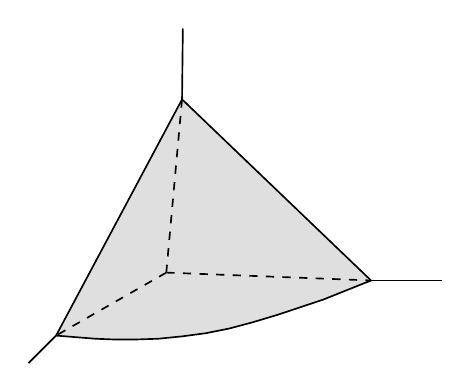
\begin{tikzpicture}[x=1cm,y=1cm,font=\normalsize,
  solidedge/.style={solid,line width=.6pt},
  dashededge/.style={dashed,line width=.6pt}]
\coordinate (O) at (2.0,2.0);
\coordinate (S) at (2.2,4.2);
\coordinate (A) at (0.6,1.2);
\coordinate (B) at (4.6,1.9);
\coordinate (Stop) at (2.21,5.1);
\coordinate (Aout) at (0.25,0.85);
\coordinate (Bout) at (5.5,1.9);
\fill[gray!25] (S) -- (A)
  -- (0.6,1.2) -- (0.85,1.18) -- (1.1,1.16) -- (1.35,1.15) -- (1.6,1.15)
  -- (1.9,1.16) -- (2.2,1.19) -- (2.5,1.23) -- (2.8,1.29) -- (3.1,1.37)
  -- (3.4,1.46) -- (3.7,1.56) -- (4.0,1.66) -- (4.3,1.78) -- (4.6,1.9)
  -- (S) -- cycle;
\draw[solidedge] (S) -- (A);
\draw[solidedge] (S) -- (B);
\draw[solidedge] (0.6,1.2) -- (0.85,1.18) -- (1.1,1.16) -- (1.35,1.15)
  -- (1.6,1.15) -- (1.9,1.16) -- (2.2,1.19) -- (2.5,1.23) -- (2.8,1.29)
  -- (3.1,1.37) -- (3.4,1.46) -- (3.7,1.56) -- (4.0,1.66) -- (4.3,1.78) -- (4.6,1.9);
\draw[solidedge] (S) -- (Stop);
\draw[solidedge] (A) -- (Aout);
\draw[solidedge] (B) -- (Bout);
\draw[dashededge] (S) -- (O);
\draw[dashededge] (O) -- (A);
\draw[dashededge] (O) -- (B);
\end{tikzpicture}
